\documentclass[pdf]{prosper}
\usepackage[utf8x]{inputenc}
\usepackage[italian]{babel}
\usepackage[capsules]{HA-prosper}
\usepackage{lscape}
\usepackage{natbib}
\title{Linguistica dei corpora: una introduzione}
\author{Luigi Talamo (talamo.luigi@gmail.com)}

\newcommand{\dxarr}{\begin{math}\rightarrow  \end{math}\hspace{1pt}}
\newcommand{\sxarr}{\begin{math}\leftarrow  \end{math}\hspace{1pt}}
\begin{document}
\maketitle

\begin{tsectionandpart}{CL: cos'è, teoria vs. metodologia, type/token, collocazione, frequenza e produttività}

\begin{slide}{Cos'è}

La linguistica dei corpora ({\it Corpus Linguistics}: CL) è lo studio del linguaggio così come lo si trova espresso in `campioni di lingua' (corpora).

Seguendo qualche suggestione naturalistica, lo possiamo paragonare all'esame dei campioni che viene effettuato nelle scienze naturali e della vita, come i campioni di sangue per la medicina e i carotaggi in geologia.

\end{slide}

\begin{slide}{Teoria o metodologia?}
	E' la domanda con cui si apre \citealt{Gries2009}, sul quale questa prima sezione è largamente basata.

Tra i linguisti dei corpora, gli approcci le risposte sono differenti:

\begin{itemize}
\item taluni, come Geoffrey Leech, considerano la CL una vera e propria `filosofia del linguaggio';
\item altri, probabilmente la maggioranza, trattano la CL come un `semplice' strumento di indagine e di analisi.
\end{itemize}

\end{slide}

\begin{slide}{CL come teoria}
Se consideriamo la CL come teoria, dovremmo poter elaborare una spiegazione al linguaggio (e di conseguenza una grammatica) guidati ({\it driven}) dai dati `grezzi' del campione linguistico.

E' l'oggetto della {\it corpus-driven linguistics}: 

\begin{itemize}
\item uno dei principali obiettivi del trattamento automatico del linguaggio è quello di insegnare alle macchine il linguaggio naturale somministrando loro grosse quantità di dati linguistici;
\item discipline più teoriche come la semantica distribuzionale cercano di catturare i significati delle parole dai contesti in cui si trovano: ``You shall know a word by the company it keeps'' (Joseph Rupert Firth)
\item ``to derive linguistic categories systematically from the recurrent patterns and the frequency distributions that emerge from language in context'' (\citealt{Togninibonelli2001}:87, citato in \citealt{JensetMcgillivray2017}:59)
\end{itemize}

\end{slide}

\begin{slide}{CL come metodologia di indagine}
Considerare la CL come `semplice' metodologia di indagine non vuol dire affatto ridurre la sua portata a `mero strumento'; tuttavia, se la CL non è teoria di per sé, a quale sistema teorico la possiamo riferire?

\begin{itemize}
	\item alcune discipline linguistiche semplicemente non si {\it curano} di avere o di esplicitare basi teoriche: la maggior parte dei dizionari contemporanei è basata su corpora linguistici, così come molte opere di linguistica applicata e didattica delle lingue;
	\item la CL è ormai lo strumento di base della linguistica cognitiva e di stampo funzionalista, cioè di una linguistica basata sull'uso effettivo che i parlanti fanno della lingua ({\it usage-based cognitive-linguistic theories}). In questo senso, la CL si oppone anche teoricamente alla linguistica di stampo generativista, che è tradizionalmente basata sull'analisi del proprio ( = del linguista) linguaggio.
\end{itemize}
\end{slide}

\begin{slide}{CL e teorie costruttiviste}
L'uso della lingua da parte dei parlanti è uno dei pilastri fondamentali di una linguistica molto {\it à la page}, ovvero della linguistica di impianto costruttivista ({\it constructional grammar}). 

	Esistono almeno una mezza dozzina di teorie costruttiviste: la Construction Grammar (\citealt{Goldberg2013}), la Radical Construction Grammar (\citealt{Croft2001}), la Construction Morphology (\citealt{Booij2010}), \dots

Un altro pilastro fondamentale di queste teorie è ovviamente la costruzione, identificata come un unità fondamentale di forma e significato, che include in sé le tradizionali categorie linguistiche di morfema, parola, sintagma, ecc.

	\begin{itemize}
		\item Cagliari;
		\item cagliaritano;
		\item acchiappa-titolo;
		\item macchina da scrivere.
    	\end{itemize}

Da un punto di vista teorico la CL ha come unità fondamentale la collocazione.
\end{slide}

\begin{slide}{Type, token e collocazione}

Espressione = morfema, parola, composto, parola complessa, frase -> in CL `type'

Occorrenze = tutte le volte in cui trovo una data espressione su un corpus -> in CL `token'

Collocazione = insieme dei contesti di un corpus in cui si trova una data espressione, cioè insieme delle occorrenze

	Esempio: 188 token del type `rebbio' sul corpus ItWac (circa 1 miliardo di token)

\begin{center}
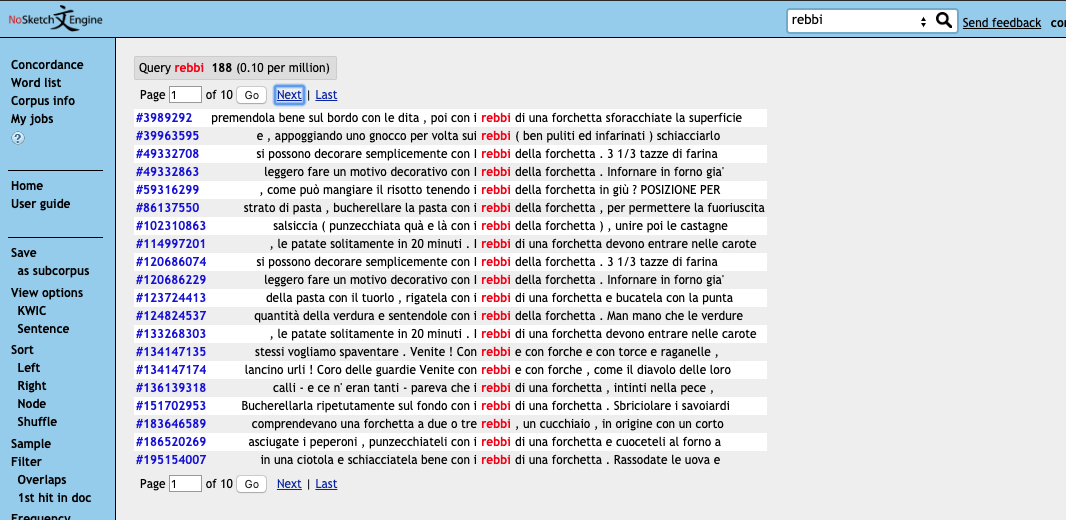
\includegraphics[width=11cm]{rebbio}
\end{center}

\end{slide}

\overlays{5}{
\begin{slide}{Collocazioni di {\it rebbio}}
Cosa scopriamo dalle collocazioni di {\it rebbio} viste sopra? Abbastanza!

\begin{itemstep}
\xitemwait
\xitem è un nome, compare, tranne che in due casi, solo al plurale e spesso nel caso strumentale;
\xitem è spesso modificato da `una forchetta';
\xitem è retto da verbi che hanno a che fare con il campo semantico della cucina: `bucherellare', `punzecchiare', \dots;
\xitem più in generale, si trova vicino a nomi e verbi che denotano questo campo semantico: melanzana, spennellare, \dots;
\end{itemstep}

La collocazione di una espressione ci svela le sue caratteristiche grammaticali (formali) e il suo significato, proprio come la costruzione è la rappresentazione della forma e del significato di una espressione.


\end{slide}
}

\overlays{5}{
\begin{slide}{Frequenza}
Nella sua accezione più semplice, la frequenza è la somma aritmetica delle collocazioni, cioè: l'espressione X si trova Y nel corpus Z.

\begin{itemstep}
\xitemwait
\xitem auto di piazza: ?
\xitem non la conosco: tre espressioni distinte. Auto che si prende in piazza? A noleggio?
\xitem 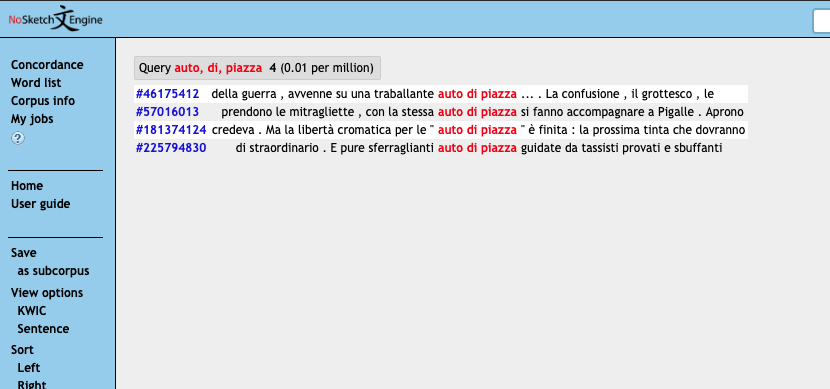
\includegraphics[width=11cm]{autodipiazza}
\xitem ora la conosco: una unica espressione (`parola') con tre token in ItWac
\end{itemstep}
\end{slide}
}

\begin{slide}{Frequenza come {\it entrenchment}}
	Il concetto di frequenza è nuovamente un concetto che ha un corrispettivo funzionale nella linguistica cognitiva.
	
	Più alta è la frequenza, maggiore è la possibilità che una data costruzione sia immagazzinata (radicata) nel lessico mentale dei parlanti.

	\begin{itemize}
		\item se l'espressione è immagazzinata nel lessico, non la devo scomporre: <auto di piazza>;
		\item se non è immagazzinata, la devo analizzare `al volo': <auto> <di> <piazza>.

	\end{itemize}
\end{slide}

\end{tsectionandpart}

\begin{tsectionandpart}{CL al lavoro: qualche applicazione}

	\overlays{3}{
\begin{slide}{Annotazioni: lemma e PoS}
	Negli esempi fatti fino ad ora abbiamo interrogato il nostro corpus direttamente in base alla parola. Un corpus linguistico può offrire però molto di più, potendo essere annotato a tutti i livelli di analisi linguistica. Per ora vediamo le due principali annotazioni, quelle presenti `di default' (o quasi...) su ogni corpus:

	\begin{itemstep}
	\xitemwait
	\xitem lessicografica, indicando cioè il lemma o `forma di citazione'; ad es., i token `rosolerà', `rosolino', `rosolavano' sono forme dello stesso lemma ROSOLARE;
	\xitem sintattica. In base ad un insieme di etichette finito e specifico per ogni corpus ({\it tagset}), ciascun token è annotato per classe di parola (categoria lessicale, parte del discorso: {\it Parts of Speech}: PoS) ed eventuali altre caratteristiche morfo-sintattiche; ad., il verbo `rosolino' è annotato nel {\it tagset} di ItWac come verbo finito: VER:fin
	\end{itemstep}
\end{slide}
	}

\begin{slide}{Annotazioni: il corpus come tabella}
Possiamo immaginare un corpus linguistico come una gigantesca tabella, le cui linee corrispondono ai token e le colonne alle annotazioni. 
\begin{center}
\begin{tabular}{c|c|c}
	WORD &	PoS &	LEMMA \\
	La &	ART &	la \\
	nebbia &	NOUN &	nebbia \\
	agli &	ARTPRE &	al \\
	irti &	ADJ &		irto \\
	colli &	NOUN &	colle|collo \\
	piovigginando &	VER:geru &	piovigginare \\
	sale &	NOUN &	sala|sale \\
	, &	PUN &	, \\
\end{tabular}
\end{center}

La prima colonna di solito coincide con WORD, ma è di fatto una convenzione.

Trova l'errore!

\end{slide}

\begin{slide}{Annotazioni: come utilizzarle}
Le annotazioni possono essere combinate nella nostra ricerca, al fine di ottenere dei risultati più raffinati.
Concettualmente, questo equivale a scegliere le righe di una tabella filtrandole attraverso una o più colonne.

Ad es., `Dammi tutte le righe in cui compare un nome', `Dammi tutte le righe in cui NON compare un verbo', `Dammi tutte le righe in cui compare un nome al plurale in -i'.

Una operazione che può essere fatta semplicemente attraverso un foglio di calcolo come Excel o Numbers: tuttavia, questo non è né computazionalmente ottimale né umanamente efficace, soprattutto se ci troviamo di fronte a corpora con milioni di token ( = milioni di righe!) e dozzine di annotazioni ( = dozzine di colonne).

Inoltre, richieste del tipo `Dammi tutte le righe in cui nome compare insieme ad un aggettivo' sono difficili da soddisfare con un programma che ragiona solo per colonne...

\end{slide}

\begin{slide}{Maschere di ricerca}
	Molti corpora dispongono di una interfaccia grafica, con una comoda maschera di ricerca dove effettuare le proprie query. Utilizzeremo come software di ricerca NoSketch Engine, la cui maschera di ricerca consente di ricercare sia espressioni formate da un solo token (simple) che da più di un token (phrase).

Purtroppo ci sono dei limiti:

\begin{itemize}
\item è possibile cercare solo per alcuni tipi di annotazione: token e lemma;
\item non è possibile combinare più di un tipo di annotazione per lo stesso token. Ad es., non è possibile una ricerca come `token = sveglia e PoS = aggettivo';
\item è possibile combinare due token solo selezionando il secondo token come lemma. Ad es., è possibile combinare il token `cipolla' solo con il lemma `rinvenire', ma non, ad esempio, con una parte del discorso come `verbo'.
\end{itemize}
\end{slide}

\begin{slide}{Corpus Query Language}
Il modo più efficace per interrogare un corpus è attraverso uno speciale linguaggio, il Corpus Query Language (CQL), originariamente creato all'inizio degli anni '90 per uno dei primi software di interrogazione, il Corpus Query Processor (CQP).

CQL è `parlato' da diversi software di interrogazione e utilizzato da molti corpora: è il linguaggio con cui si può interrogare Sketch Engine, un software commerciale che include 500 corpora pre-caricati per più di 90 lingue. 
	
Essendo NoSketch Engine l'implementazione {\it open source} di Sketch Engine, CQL `funziona' anche su questo software!

\end{slide}

\begin{slide}{Corpus Query Language: l'unità di base}
L'unità di base di CQL è la seguente:

\begin{center}
\begin{verbatim}
[attributo="valore"]
\end{verbatim}
\end{center}

dove ciascun token è racchiuso tra due parentesi quadre e `attributo' sta per qualsiasi tipo di annotazione: word, PoS, lemma.

Per cercare espressioni formate da più token, ad esempio `la cipolla rinviene', ripeteremo dunque questa unità di base:

\begin{center}
\begin{verbatim}
[attributo="valore"] [attributo="valore"] [...]
\end{verbatim}
\end{center}

\end{slide}

\begin{slide}{Corpus Query Language: le espressioni regolari}
CQL può utilizzare le cosidette `espressioni regolari' ovvero simboli speciali che possono essere utilizzati per cercare delle sequenze di caratteri piuttosto che caratteri singoli.

Alternanza di caratteri nella parola. Ad esempio, vogliamo cercare le forme femminili e maschili di `gatto':

\begin{center}
\begin{verbatim}
[word="gatt[ao]"]
\end{verbatim}
\end{center}

Qualsiasi carattere nella parola. Ad esempio, vogliamo cercare in quali modi è flesso il nome `dito':

\begin{center}
\begin{verbatim}
[word="dit."]
\end{verbatim}
\end{center}

Qualsiasi sequenza di caratteri (alla fine o all'inizio della parola). 
	
Ad esempio, vogliamo cercare tutte le parole in `poli':

\begin{center}
\begin{verbatim}
[word=".*poli$"]
\end{verbatim}
\end{center}

oppure che iniziano con `tele':

\begin{center}
\begin{verbatim}
[word="^tele.*"]
\end{verbatim}
\end{center}

\end{slide}
\begin{slide}{Corpus Query Language: combinare le annotazioni}
Possiamo infine combinare le annotazioni all'interno dello stesso token. Ad esempio, possiamo cercare tutte le occorrenze di `sveglia' come aggettivo:

\begin{center}
\begin{verbatim}
[lemma="sveglio" & tag="ADJ"]
\end{verbatim}
\end{center}

dove ciascun token è racchiuso tra due parentesi quadre e `attributo' sta per qualsiasi tipo di annotazione: word, PoS, lemma.

\end{slide}

\overlays{5}{
\begin{slide}{Oltre il lessico}
	Oltre al lessico, che è il primo, tradizionale dominio di utilizzo della CL (ad es., i progetti lessicografici avviati dal De Mauro dagli anni settanta già utilizzavano dei corpora), la CL trova impiego in moltissimi altri campi legati alle scienze linguistiche:

	\begin{itemstep}
	\xitemwait 
	\xitem abbiamo già menzionato sopra dizionari e usi didattici della CL;
	\xitem calcolare la produttività di una costruzione morfologica;
	\xitem predirre quali scelte sintattiche fanno i parlanti di una lingua (e perché): ad es., il congiuntivo italiano è veramente morto?
	\xitem identificare il reale utilizzo di due parole all'apparenza tra loro sinonimiche: es. di sopra, quando utilizziamo {\it auto di piazza} al posto di `taxi'?
	\end{itemstep}
	\end{slide}
}

\begin{slide}{Costruzioni morfologiche: frequenza e produttività}
Facciamo ora il caso delle costruzioni morfologiche di tipo derivazionale, come le prefissazioni e le suffissazioni. Ad es., quanto e come i parlanti di lingua italiana utilizzano

	\begin{itemize}
		\item il suffisso {\it -ame}? legname, pietrame, bambiname, berlusconame, grillame 
		\item il prefissoide {\it tele-}? televendita, telecomando, telepresentatore
		\item il suffisoide {\it -poli}? tangentopoli, vallettopoli, guerciopoli
		\item il primo membro del composto {\it acchiappa-}? acchiappa-macchie, acchiappa-titoli
	\end{itemize}


ovvero: quanto e come è produttiva una data costruzione?

\end{slide}

\begin{slide}{Costruzioni morfologiche: type/token}
	Definire la frequenza e la produttività di una costruzione morfologica è un compito leggermente diverso dal definire gli stessi valori per una parola come {\it rebbi} o {\it auto di piazza}.

Abbiamo detto prima che in CL una parola equivale ad un type, di cui troviamo un certo numero di token in un corpus.

Nelle costruzioni morfologiche ci troviamo di fronte a una regola - la costruzione, appunto - che crea:

	\begin{itemize}
	\item un certo numero di type diversi;
	\item ciascuno di questi type mostra un certo numero di token.
	\end{itemize}
\end{slide}

\begin{slide}{Tre tipi di produttività morfologica}
Per quanto riguarda le costruzioni morfologiche, \citealt{Baayen2009} distingue tre tipi di produttività:

	\begin{enumerate}
		\item produttività realizzata;
		\item produttività in espansione;
		\item produttività potenziale.
	\end{enumerate}	

\end{slide}

\begin{slide}{Produttività realizzata}
La produttività realizzata è il tipo più semplice di produttività e coincide di fatto con la frequenza dei types di una determinata costruzione morfologica.

Volendo fare un'analogia con l'economia, il primo tipo di produttività è simile alla fetta che ha una compagnia detiene sul mercato.

Se la produttività realizzata è alta, la costruzione morfologica avrà una grossa quota consolidata nel `mercato' delle derivazioni morfologiche.


	\begin{itemize}
		\item Come si calcola: Numero di types (costruzione)
	\end{itemize}

\end{slide}

\begin{slide}{Produttività in espansione}
Nel nostro paragone con l'economia di mercato, il secondo tipo di produttività misura quanto la costruzione morfologica si sta espandendo, anche a danno di altre derivazioni morfologiche. 

E' inoltre interessante notare che una costruzione può avere una scarsa produttività realizzata, ma un'alta produttività in espansione -> è il caso dei nuovi affissi

	\begin{itemize}
		\item Come si calcola. P = numero di hapax legomena (costruzione) / numero di hapax legomena (corpus)
	\end{itemize}

\end{slide}

\begin{slide}{Produttività potenziale}
Il terzo tipo di produttività misura quanto una costruzione morfologica è in grado di occupare una fetta di mercato; una azienda può essere anche in espansione, ma se il mercato è ormai saturo rischia probabilmente di fare bancarotta!

E' il tipo di produttività più utilizzato negli studi di CL e morfologia quantitativa, ed è chiamato semplicemente P:

\begin{itemize}
\item Come si calcola. P = numero di hapax legomena (costruzione) / numero di token totali (costruzione)
\end{itemize}

Con un aggiustamento a livello di sotto-corpora, l'indice P è utilizzato nei lavori di Gaeta \& Ricca sulla produttività dei suffissi italiani (\citealt{GaetaRicca2003}, \citealt{GaetaRicca2006}).
\end{slide}

\begin{slide}{Costruzioni morfologiche: esercizio}
Data la (reale) lista di frequenza della costruzione con {\it -ame} nel corpus La Repubblica, calcolare i tre tipi di produttività.

\end{slide}

\begin{slide}{Costruzioni sintattiche: type/token}
Secondo il principio di non sinonimicità, una differenza formale tra due costruzioni implica SEMPRE una differenza di significato: ``If two constructions are syntactically distinct, they must be semantically or pragmatically distinct'' (Adele Goldberg)

Per quanto riguarda la sintassi, possiamo dunque decidere di studiare in CL una costruzione che può essere espressa in diversi modi formali (type), ciascuno dei quali mostrerà un certo numero di token.

\end{slide}

\overlays{8}{
\begin{slide}{Costruzioni sintattiche: la costruzione ditransitiva inglese}
	Ad es., l'inglese esprime la costruzione ditransitiva:

	\begin{itemstep}
	\xitemwait 
	\xitem Funzione: trasferire qualcosa a qualcuno;
	\xitem ruoli semantici/argomentali: AGENT TRANSFER PATIENT RECIPIENT
	\xitem	dove TRANSFER è un verbo come {\it to give}, {\it to bring}, {\it to tell}, {\it to play}.
	\xitem in due modi sintatticamente diversi, cioè in due ruoli grammaticali/sintattici diversi:
	\xitem SUBJ TRANSFER DIRECT-OBJECT INDIRECT-OBJECT: Mary gives a letter to John;
	\xitem SUBJ TRANSFER DIRECT-OBJECT DIRECT-OBJECT:Mary gives John a letter.
	\xitem marcando cioè in modo diverso il RECIPIENT
	\end{itemstep}
\end{slide}
}

\begin{slide}{Costruzioni sintattiche: esercizio}
Data la (reale) lista di frequenza delle realizzazioni sintattiche della costruzione ditransitiva 
	
	\begin{itemize}
		\item con quattro verbi inglesi: give, bring, tell, play
		\item ciascuno nella variante con oggetto diretto o con oggetto indiretto
	\end{itemize}

quali caratteristiche semantiche e funzionali possiamo dedurre dalla distribuzioni di questi otto types sintattici?

\end{slide}
\end{tsectionandpart}

\begin{tsectionandpart}{Creazione di un corpus testuale}

\begin{slide}{Tabella di marcia}
\begin{center}
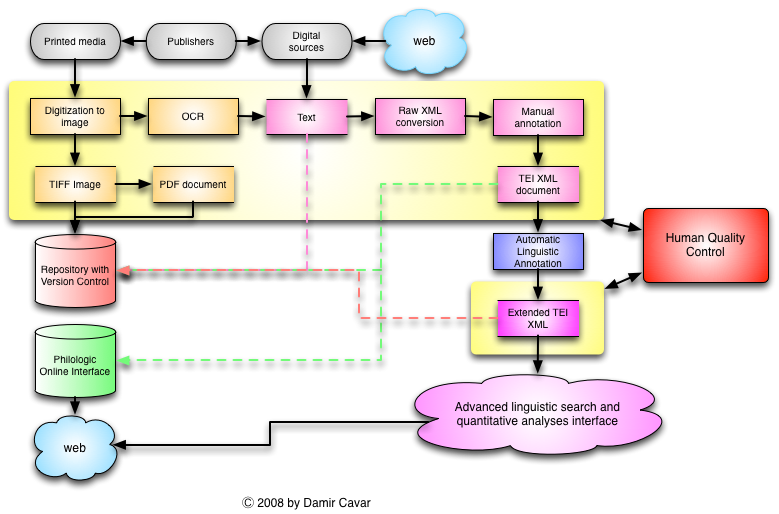
\includegraphics[width=11cm]{corpusprocess}
\end{center}
\end{slide}

\begin{slide}{Annotazione del linguaggio}
\begin{center}
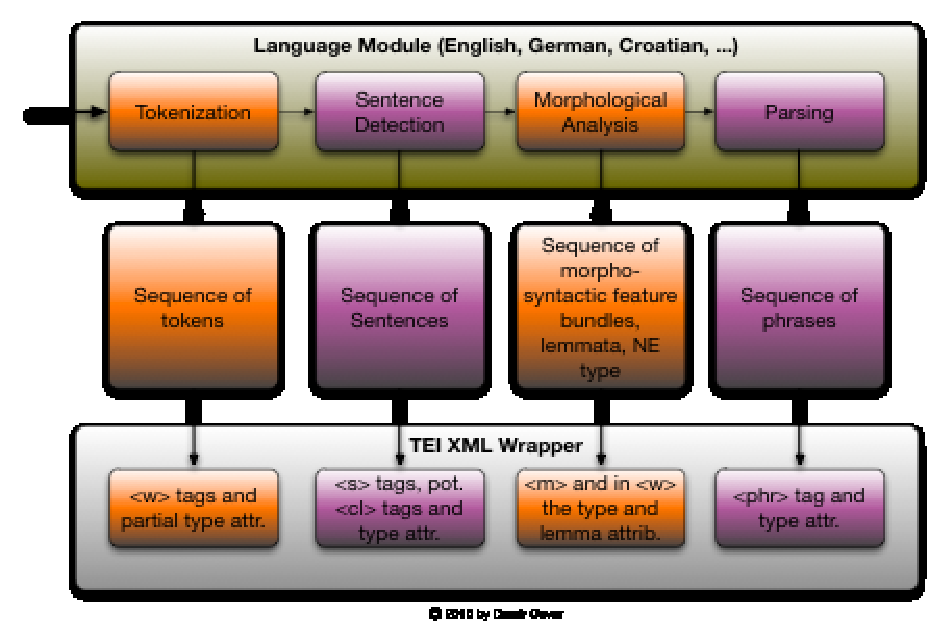
\includegraphics[width=11cm]{langproc}
\end{center}
\end{slide}

\begin{slide}{Annotazione posizionale}
Si applica al singolo token e funziona con il modello a colonna:
	\begin{verbatim}
	In	PRE	in
	periferia	NOUN	periferia
	fa	VER:fin	fare
	molto	ADV	molto
	caldo	ADJ	caldo
	/	PUN	/
	mamma	NOUN	mamma
	stai	VER:fin	stare
	tranquilla	ADJ	tranquillo
	,	PUN	,
	sto	VER:fin	stare
	arrivando	VER:geru	arrivare
	\end{verbatim}
	
	Ma come fare ad annotare espressioni con più di un token, ad esempio l'espressione `auto di piazza' o `rebbi della forchetta'?
\end{slide}

\begin{slide}{Annotazione strutturale}
L'annotazione strutturale `copre' più di un token e viene implementata attraverso un linguaggio di {\it markup}. Il linguaggio più utilizzato è XML, disponibile in vari `dialetti'.


	\begin{verbatim}
	<?xml version="1.0" encoding="UTF-8" ?>
	<text num="1" title="Soldi" author="Mahmood">
	<l>
	In	PRE	in
	periferia	NOUN	periferia
	fa	VER:fin	fare
	molto	ADV	molto
	caldo	ADJ	caldo
	</l>
	</text>
	\end{verbatim}

Per codificare un testo linguistico il dialetto XML più utilizzato è lo standard TEI: {\it Text Encoding Initiative}.

\end{slide}

\begin{slide}{Annotazione TEI-XML: struttura di base}
Le annotazioni XML possono in realtà coprire tranquillamente il singolo token, che viene annidato assieme ad altri token in strutture più complesse come i sintagmi, i versi/frasi, fino ad arrivare al testo:

\begin{verbatim}
<?xml version="1.0" encoding="UTF-8"?>
<TEI xmlnsoff="http://www.tei-c.org/ns/1.0">
<teiHeader>
</teiHeader>
<text>
<body>
<l>
<tok id="w-1" pos="PRE" lemma="in">In</tok>
<tok id="w-2" pos="NOUN" lemma="periferia">periferia</tok>
...
</l>
</body>
</text>
\end{verbatim}
\end{slide}

\begin{slide}{Il TEI-Header}
Questa sezione comprende informazioni di carattere metalinguistico e che riguardano tutto il testo. Come tutti i tag XML, anche il TEI-Header fa ampio uso del concetto di gerarchia, cioè di tag annidati dentro altri tag:

	\begin{itemize}
	\item <fileDesc><titleStmt><title>...</title></titleStmt></fileDesc>: titolo del testo;
	\item <fileDesc><titleStmt><author>...</author></titleStmt></fileDesc>: l'autore del testo;
	\item  <fileDesc><publicationStmt><publisher>...</publisher></publicationStmt></fileDesc>: chi ha pubblicato il testo;
	\item <profileDesc><textClass>...</textClass></profileDesc>: tipo di testo.
	\end{itemize}



\end{slide}
\end{tsectionandpart}
	
\bibliography{ref}
\bibliographystyle{natbib}
\end{document}
